% moved to iteracion 2


% \section{Ruta óptima dentro el Campus Universitario}
% \label{sec:generar_mapa_rutas}

Para poder responder al problema de encontrar una ruta óptima entre 2 puntos dentro del campus universitario, se necesita de un mapa que contenga todas las rutas que existen dentro del campus.\\

 %
 %
 % \section{Campus Universitario}
 % \label{sec:ruta_corta_umss}

 En primer lugar fue necesario obtener un grafo ponderado no-dirigido que representa un mapa de los caminos que existen dentro del campus Universitario.\\

 Para obtener este mapa se procedió a caminar a través del campus de la UMSS con un GPS Garmin Nuvi 1300, el cual es un dispositivo GPS básico pero cumple con la función de guardar información geográfica, los archivos generados tienen extensión \emph{gpx}, que básicamente es un fichero XML estándar usado para compartir datos entre GPS's, se recorrieron los principales caminos que existen e interconectan las distintas facultades y oficinas dentro del campus universitario. Una vez realizado este recorrido, se procedió a extraer la información del dispositivo GPS, se utilizó el archivo \emph{current.gpx} para exportar la información  a un archivo \emph{shapefile}, para esta tarea se utilizó QGis, con el cual se acabó editando las rutas recogidas por el GPS.\\

% \footnote{Un shapefile es un archivo de formato sencillo y no topológico que se utiliza para almacenar la ubicación geométrica y la información de atributos de las entidades geográficas.\cite{what_is_shapefile} }

 Este paso fue necesario porque el mapa extraído del GPS es una línea única, pero para que nos sirva para el objetivo de buscar una ruta óptima, es necesario que esta línea sea dividida o separada en muchas líneas, las cuales son las aristas y los extremos de las líneas serán los nodos o vértices del grafo.\\

 Implementando el algoritmo de \emph{Dijkstra} en el grafo resultante es lo que nos permitir\'a encontrar la ruta más corta dentro del campus Universitario, al tener una gran cantidad de información resultante de la obtención de datos mediante un dispositivo GPS se hace imprescindible usar una base de datos que nos ayude con esta tarea, para lo cual se usó la base de datos PostgreSQL añadiendolo PostGIS y pgRouting, herramientas ampliamente utilizadas en el manejo de datos geo-espaciales.\\

  % el grafo representa el mapa de caminos  pueda ser usado en una base de datos  “ruteable”, esto significa que el mapa de una sola línea hay que separarlo o dividirlo en muchas líneas.\\


 Técnicamente esta línea única es representada como un \emph{POLYLINE} el cual consiste en una o más partes. Una parte es una secuencia conectada de dos o más puntos. Las partes pueden o no estar conectadas entre sí. Las partes pueden o no intersectarse entre sí, para transformar este POLYLINE necesitamos separar todas sus partes y convertirlas en objetos \emph{LINESTRING} únicos, y a este conjunto de LINESTRINGs es el que se va a usar en la base de datos como mapa de ``rutas''.\cite{esri_shapefile}\\

 \begin{figure}[H]
   \begin{center}
     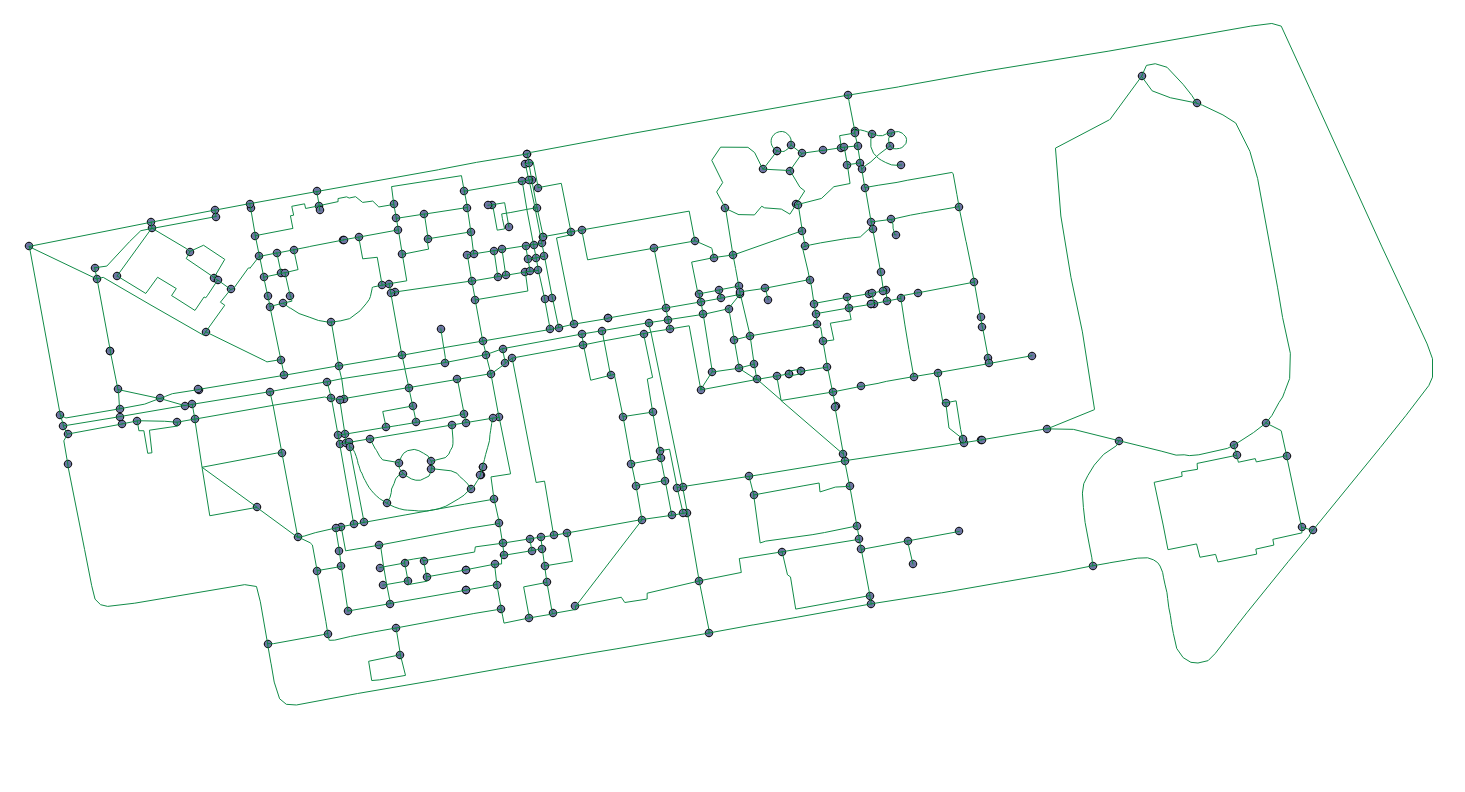
\includegraphics[width=1\textwidth]{shapefile_umss_v1}
     \caption{Shapefile del campus Universitario.}
     \label{fig:shapefile_umss_v1}
     \caption*{Fuente: Elaboración propia}
   \end{center}
 \end{figure}

 En la figura \ref{fig:shapefile_umss_v1} se puede apreciar el shapefile resultante de la división del POLYLINE original, las líneas que conforman el mapa de las rutas del campus Universitario, donde cada línea es una arista y los puntos son los nodos del grafo no-dirigido, que será usado para la resolución del problema de la ruta más corta en el presente proyecto de grado.\\
 %
 % Para una mejor apreciación del grafo que consta de 1164 aristas y 1003 vértices, se lo puede ver en combinación o proyectada en un mapa de rutas del campus de la Universidad Mayor de San Simón ubicado entre las calles Oquendo, Sucre y  Belzu de la ciudad de Cochabamba - Bolivia, se puede referir a la siguiente figura \ref{fig:shapefile_umss_v2}.
 %
 % \begin{figure}[H]
 %   \begin{center}
 %     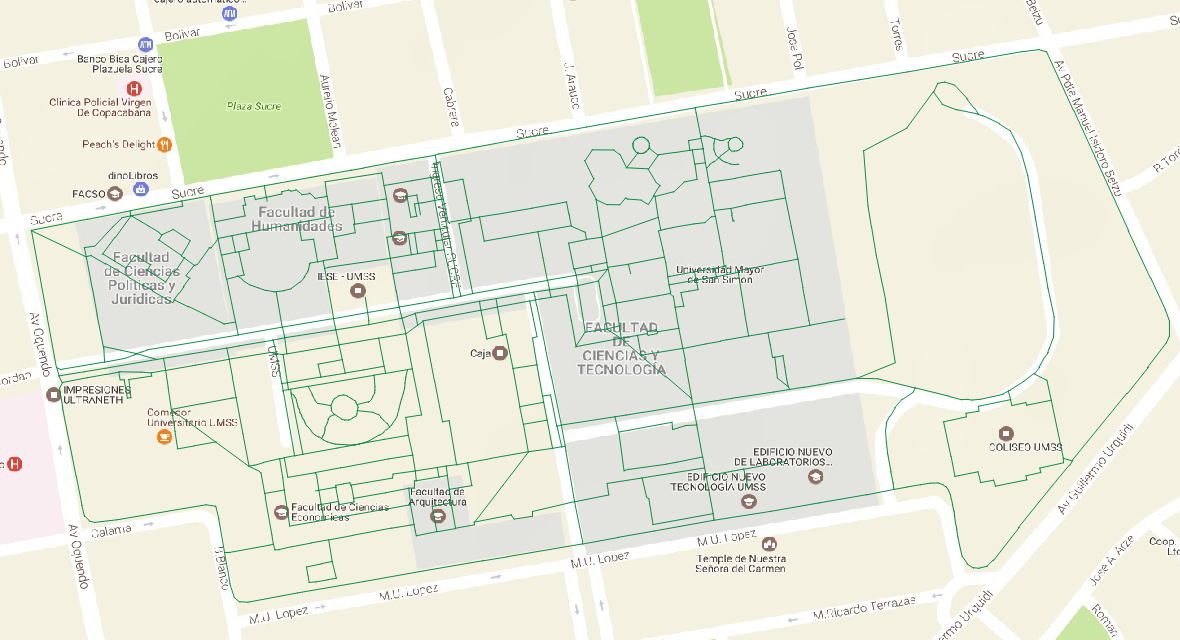
\includegraphics[width=1\textwidth]{shapefile_umss_v2}
 %     \caption{Shapefile sobre el campus Universitario de la UMSS.}
 %     \label{fig:shapefile_umss_v2}
 %     \caption*{Fuente: Elaboración propia}
 %   \end{center}
 % \end{figure}


 % moved to iteracion 2
